\documentclass[11pt]{article}
\usepackage[T1]{fontenc}
\usepackage[utf8]{inputenc}
\usepackage{lmodern}
\usepackage[margin=2.3cm]{geometry}
\usepackage{booktabs,longtable,array,graphicx,amsmath,url,hyperref,float,caption,enumitem}
\usepackage{color}
\renewcommand{\arraystretch}{1.08}
\newcolumntype{L}[1]{>{\raggedright\arraybackslash}p{#1}}
\graphicspath{{figures/}}
\hypersetup{colorlinks=true,linkcolor=blue,urlcolor=blue,citecolor=blue}

\title{\textbf{SmogShield Lahore}\\[2mm]
Deliverable 2: Phase 3 (Model Development) and Phase 4 (Evaluation and Bias Analysis)}
\author{Muhammad Haider Mughal (3006) \and Muhammad Ayub Butt (3076) \and Abdul Rehman (3059)}
\date{9 November 2026}

\begin{document}
\maketitle

\begin{abstract}
This report documents the Deliverable 2 work for SmogShield and covers Phase 3 (model development) and Phase 4 (evaluation and bias analysis). The primary task is six-class next-day AQI-category classification; the secondary task is next-day PM2.5 regression. All experiments use one chronological split, a seven-day purge gap, train-only preprocessing, and a test set touched once per final model. The selected classifier, HistGradientBoosting, achieved a validation macro F1 of 0.4941 and a test macro F1 of 0.4780. It did not beat the persistence baseline on test (0.5157), although its accuracy was slightly higher (0.5856 versus 0.5676). For regression, HistGradientBoosting was selected on validation RMSE (45.6243 versus Ridge 45.6916); its test RMSE was 64.9198, essentially tied with persistence (64.8175, a 0.10 gap and skill $-0.0016$). Ridge did beat persistence on test with RMSE 62.0956. The bias analysis shows especially large errors on the most severe pollution days; because severity groups are defined by the observed outcome, the sign is partly constructed, and the error magnitude is the informative result. The report states these results as observed rather than tuning the test set after the fact.
\end{abstract}

\tableofcontents

\section{Introduction and objectives}

SmogShield forecasts next-day air quality for Lahore, Pakistan. The modelling work has two tasks:

\begin{enumerate}[leftmargin=1.4em]
  \item \textbf{Primary:} predict the next-day AQI category among six classes (Good/Moderate, Unhealthy for Sensitive, Unhealthy, Very Unhealthy, Hazardous 301--400, and Hazardous 401--500).
  \item \textbf{Secondary:} predict next-day PM2.5 concentration as a continuous value.
\end{enumerate}

The primary task supports the classification analysis required for the project: accuracy, balanced accuracy, macro precision, macro recall, macro F1, weighted F1, one-vs-rest macro AUC-ROC, a confusion matrix, and per-class precision/recall/F1. Macro metrics are primary because the classes are imbalanced. The regression task reports RMSE, MAE, and $R^2$, and compares every model with a persistence baseline.

The guiding rule is that tomorrow's value is unknown at forecast time. Only today's PM2.5, AQI, weather, and calendar information may be used as model inputs. No feature may be derived from \texttt{shift(-1)} or from the test period.

\subsection{Phase coverage}

This report is the Deliverable 2 submission for Phase 3 and Phase 4. Sections~4--6 cover Phase~3: the model and baseline protocol, classification results, and regression results. Sections~7--10 cover Phase~4: bias and error analysis, limitations and recommendations, reproducibility, and conclusions. Sections~2--3 document the shared data and preprocessing contract that both phases depend on, and Section~1.2 gives the architecture.

\subsection{System architecture}

Figure~\ref{fig:architecture} summarises the Deliverable 2 path from raw sources to the report. Phase 2 cleaning and feature building produce the shared daily table. The shared loader applies the chronological split, the Good/Moderate label merge, train-only preprocessing, leakage guards, and the scorable-row mask. Classification and regression then run as separate model tracks. Their final predictions feed the shared metrics, the bias/error analysis, the frozen output files, and the report. A future application layer would consume the same forecasts and charts; it would not retrain models. The web application itself is future work and is not part of this deliverable.

\begin{figure}[htbp]
  \centering
  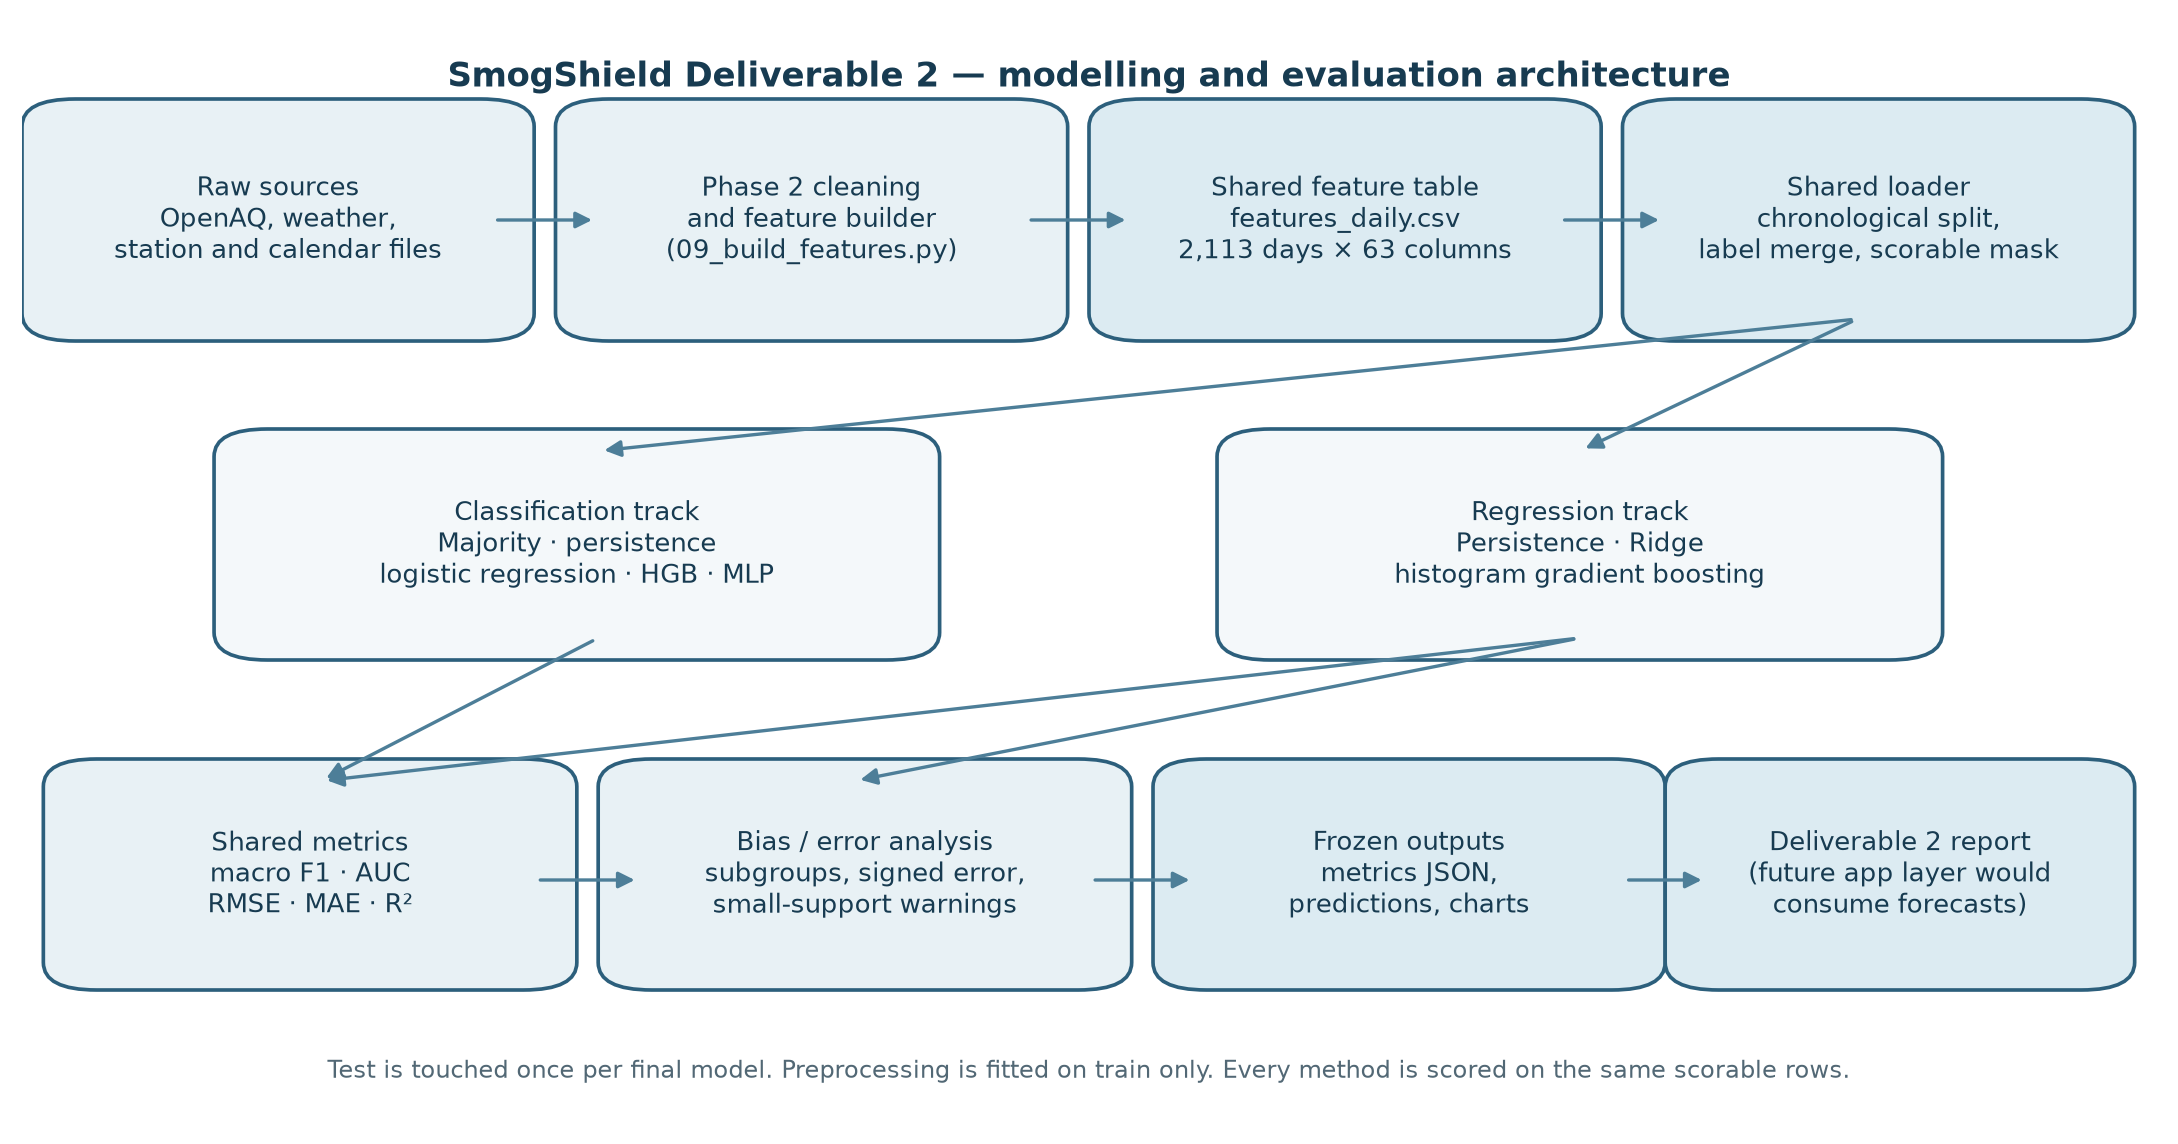
\includegraphics[width=\linewidth]{architecture.png}
  \caption{Deliverable 2 modelling and evaluation architecture. The shared loader is the single source of split, label, preprocessing, and scorable-row rules. The application forecasts shown in the last box are future work and are not part of Deliverable 2.}
  \label{fig:architecture}
\end{figure}

\section{Data and chronological split}

The shared input table is \texttt{data/processed/features\_daily.csv}. It contains 2,113 daily rows and 63 columns. It is generated by the Phase 2 feature script and is not committed to Git; it must be restored from the shared Drive or regenerated. The final run used the following split.

\begin{table}[htbp]
\centering
\small
\caption{Chronological split with a seven-day purge gap. Scorable rows require a finite current-day PM2.5 value.}
\label{tab:split}
\begin{tabular}{llrrrr}
\toprule
Split & Start & End & Rows & Scorable & Gap \\
\midrule
Train & 2019-05-23 & 2023-06-30 & 1,022 & 917 & 7 \\
Validation & 2023-07-14 & 2024-06-03 & 250 & 244 & 7 \\
Test & 2024-07-08 & 2025-02-16 & 223 & 222 & 7 \\
\bottomrule
\end{tabular}

\end{table}


The split is chronological, not random. The seven-day gap removes 2023-07-01 through 2023-07-07 and 2024-07-01 through 2024-07-07 so that a next-day target at the end of one period cannot overlap the first rows of the next period. The validation end is 2024-06-03 rather than the configured 2024-06-30 because the remaining June rows do not have a usable next-day target. This is expected.

The split contains 1,022 training rows, 250 validation rows, and 223 test rows. The scorable-row mask, which requires a finite current-day PM2.5 value, leaves 917 training rows, 244 validation rows, and 222 test rows. All methods, including persistence, are scored on the same scorable rows. Six validation rows and one test row are dropped for this reason. Classification and regression each produce 473 prediction rows (250 validation plus 223 test), of which 466 are scorable.

\subsection{Target merge and class support}

The raw table has seven AQI categories. Good has only nine training rows and zero validation and test rows, so it cannot support a separate class. For modelling, Good is merged into Moderate. This is a label decision, not a deletion: the raw category table still contains all seven categories.

\begin{table}[htbp]
\centering
\small
\caption{Raw category counts before the Good-to-Moderate merge.}
\label{tab:raw-counts}
\begin{tabular}{lr}
\toprule
Raw AQI category & Days \\
\midrule
Good & 9 \\
Moderate & 126 \\
Unhealthy for Sensitive & 269 \\
Unhealthy & 647 \\
Very Unhealthy & 256 \\
Hazardous (301-400) & 139 \\
Hazardous (401-500) & 60 \\
Total & 1,506 \\
\bottomrule
\end{tabular}

\end{table}


After the merge, the six-class support is shown below. Every class has support in every split, so multiclass AUC-ROC is defined. The eight test rows in Good/Moderate and the eleven validation rows in Hazardous 401--500 are small; their per-class precision and recall are noisy, not precise estimates. The two Hazardous bands remain separate in the main analysis.

\begin{table}[htbp]
\centering
\small
\caption{Six-class support by chronological split. Good and Moderate are merged for modelling.}
\label{tab:support}
\begin{tabular}{lrrrr}
\toprule
AQI category & Train & Validation & Test & Total \\
\midrule
Good/Moderate & 109 & 16 & 8 & 133 \\
Unhealthy for Sensitive & 175 & 53 & 34 & 262 \\
Unhealthy & 488 & 80 & 77 & 645 \\
Very Unhealthy & 148 & 47 & 61 & 256 \\
Hazardous (301-400) & 72 & 43 & 24 & 139 \\
Hazardous (401-500) & 30 & 11 & 19 & 60 \\
Total & 1,022 & 250 & 223 & 1,495 \\
\bottomrule
\end{tabular}

\end{table}


Table~\ref{tab:raw-counts} counts the current-day AQI category over all feature-table rows, while Table~\ref{tab:support} counts next-day targets inside the chronological splits. Their totals therefore differ (1,506 versus 1,495).

\section{Features, leakage controls, and preprocessing}

The shared loader drops \texttt{date}, every \texttt{target\_next\_*} column, the precomputed \texttt{*\_scaled} weather columns, the redundant \texttt{season} string, and \texttt{year} from model inputs. The last choice avoids asking trees to extrapolate to unseen years and avoids unstable linear year trends. Month, day-of-year, and cyclical encodings carry seasonality.

The loader keeps current-day PM2.5, AQI, weather, and calendar features. It one-hot encodes the current AQI category, median-imputes numeric features, adds missing-value indicators, and applies a robust scaler. Imputers and scalers are fitted on the training split only. In the model frames, \texttt{pm25\_lag1} is missing for 13.4\% of training rows, 4.0\% of validation rows, and 0.4\% of test rows, so missing-value indicators are retained rather than treated as pure noise. The loader also raises if a target or precomputed scaled column survives the config lists. The final transformed feature count is 80, from 46 raw features, confirmed by \texttt{check\_setup}.

The loader uses the fixed class labels in \texttt{configs/base.yaml}; labels are never inferred alphabetically from the data. This prevents validation or test labels from changing the class order. The optional label merge is applied only to the classification target, before encoding. The final run used seed 42 and train-only fitting throughout.

\section{Phase 3: Models, baselines, and selection protocol}

\subsection{Classification}

The classification candidates were:

\begin{enumerate}[leftmargin=1.4em]
  \item Majority class.
  \item Persistence: tomorrow's category equals today's category.
  \item Logistic regression with class weights.
  \item Histogram gradient boosting (HGB).
  \item An optional small MLP, retained only if it improved validation performance.
\end{enumerate}

The persistence baseline uses the majority training class code, 2 (Unhealthy), as its fallback when today's category is missing. This fallback must be stated whenever the persistence result is reported. The MLP was excluded after validation macro F1 of 0.4124 did not exceed HGB's 0.4941.

Hyperparameters were tuned with five-fold \texttt{TimeSeriesSplit} on the raw training frame, with a seven-day gap. Tuning never cross-validated on the already-preprocessed training matrix. The final model was refitted on the training split only, not on train plus validation. The test set was then touched once for the final model. The classification selection metric was validation macro F1 over all six configured labels. The CV score is computed per fold over the classes present in that fold, so it is not directly comparable with the six-label validation score; that caveat is recorded in the metrics file.

\begin{table}[htbp]
\centering
\scriptsize
\caption{Selected hyperparameters. Classification used five-fold time-series CV with a seven-day gap and selected on validation macro F1; regression selected on validation RMSE.}
\label{tab:hyperparameters}
\begin{tabular}{llL{5.0cm}L{3.2cm}l}
\toprule
Task & Model & Selected parameters & Validation metric & Status \\
\midrule
Classification & LogisticRegression & \texttt{\{"C": 0.1, "class\_weight": "balanced", "max\_iter": 500, "penalty": "l1"\}} & macro F1 = 0.4665 & completed \\
Classification & HistGradientBoosting & \texttt{\{"l2\_regularization": 0.1, "learning\_rate": 0.1, "max\_iter": 100, "max\_leaf\_nodes": 31, "min\_samples\_leaf": 10\}} & macro F1 = 0.4941 & selected \\
Classification & MLP & \texttt{\{"alpha": 0.01, "early\_stopping": true, "hidden\_layer\_sizes": [128, 64, 32], "learning\_rate": "constant", "max\_iter": 500, "n\_iter\_no\_change": 15, "validation\_fraction": 0.1\}} & macro F1 = 0.4124 & excluded \\
Regression & Ridge & \texttt{\{"alpha": 10.0\}} & RMSE = 45.6916 & not selected \\
Regression & HGB & \texttt{\{"learning\_rate": 0.05, "max\_depth": 3, "max\_iter": 200\}} & RMSE = 45.6243 & selected \\
\bottomrule
\end{tabular}

\end{table}


\subsection{Regression}

The regression candidates were persistence, Ridge regression, and histogram gradient boosting. Hyperparameters were tuned with the same five-fold time-series procedure and a seven-day gap. Model selection used validation RMSE. The selected model was refitted on training rows only and evaluated once on test. Persistence is not imputed for missing current-day PM2.5; it is scored on the same scorable rows as the models. The final code calls the metric helper with \texttt{allow\_missing=False} for every method. The option \texttt{allow\_missing=True} remains reserved for an unfiltered persistence baseline only; the persistence \texttt{n\_dropped} values are 6 validation and 1 test, the same rows on which every method is scored.

The selected regression model was HGB, with validation RMSE 45.6243; Ridge was close behind at 45.6916. The test comparison is reported in Section~\ref{sec:reg-results} without changing the selection rule.

\section{Phase 3: Classification results}
\label{sec:clf-results}

Table~\ref{tab:clf-metrics} reports validation and test metrics for the majority, persistence, logistic regression, and HGB candidates. HGB was selected on validation macro F1 (0.4941 versus 0.4665 for logistic regression). On test, HGB reached macro F1 0.4780, below persistence's 0.5157. HGB's test accuracy was higher than persistence (0.5856 versus 0.5676), but accuracy is dominated by the larger classes; macro F1 exposes the weaker performance on rare classes.

\begin{table}[htbp]
\centering
\scriptsize
\caption{Classification results on the chronological validation and test splits. Macro F1 is the selection metric.}
\label{tab:clf-metrics}
\begin{tabular}{llrrrrrrr}
\toprule
Model & Split & Acc. & Bal. acc. & Macro P & Macro R & Macro F1 & Wtd. F1 & AUC \\
\midrule
Majority class & Validation & 0.3033 & 0.1667 & 0.0505 & 0.1667 & 0.0776 & 0.1411 & -- \\
Majority class & Test & 0.3468 & 0.1667 & 0.0578 & 0.1667 & 0.0858 & 0.1786 & -- \\
Persistence & Validation & 0.5697 & 0.4760 & 0.4772 & 0.4760 & 0.4766 & 0.5691 & -- \\
Persistence & Test & 0.5676 & 0.5157 & 0.5157 & 0.5157 & 0.5157 & 0.5676 & -- \\
Logistic regression & Validation & 0.5287 & 0.4995 & 0.4775 & 0.4995 & 0.4665 & 0.5521 & 0.8842 \\
Logistic regression & Test & 0.5225 & 0.5062 & 0.4673 & 0.5062 & 0.4601 & 0.5337 & 0.8719 \\
\textbf{HGB} & Validation & 0.5943 & 0.4976 & 0.5049 & 0.4976 & 0.4941 & 0.5824 & 0.8765 \\
\textbf{HGB} & Test & 0.5856 & 0.4776 & 0.4804 & 0.4776 & 0.4780 & 0.5815 & 0.8886 \\
\bottomrule
\end{tabular}

\end{table}


The selected HGB model's test AUC-ROC is 0.8886 and logistic regression's is 0.8719. The one-vs-rest macro AUC is computed from the aligned six-column probability matrix. Rows sum to one within the helper's tolerance. The majority baseline has no probability output, so its AUC is reported as undefined rather than filled with a fake value. HGB's test AUC (0.8886) is higher than its validation AUC (0.8765) even though its test macro F1 is below persistence. AUC measures probability ranking rather than the thresholded label decision, and persistence has no probability output, so the two metrics answer different questions. Persistence's test macro precision, recall, and F1 are all 0.5157, and its weighted F1 equals accuracy (0.5676), because predicted and true class counts coincide exactly on the test rows. This is not a copy error; it is a property of the persistence shift on this series.

Table~\ref{tab:clf-per-class} gives the selected HGB model's test per-class results. Good/Moderate has support 8 and Hazardous 401--500 has support 19; both should be read as noisy. The largest class, Unhealthy, has F1 0.7013, while Very Unhealthy has F1 0.7040. The two Hazardous bands are weaker: 0.3600 and 0.2353.

\begin{table}[htbp]
\centering
\small
\caption{Per-class test performance of the selected HistGradientBoosting classifier. Good/Moderate and Hazardous (401--500) have small support and should be treated as noisy estimates.}
\label{tab:clf-per-class}
\begin{tabular}{lrrrr}
\toprule
Category & Support & Precision & Recall & F1 \\
\midrule
Good/Moderate & 8 & 0.3750 & 0.3750 & 0.3750 \\
Unhealthy for Sensitive & 34 & 0.5161 & 0.4706 & 0.4923 \\
Unhealthy & 77 & 0.7013 & 0.7013 & 0.7013 \\
Very Unhealthy & 60 & 0.6769 & 0.7333 & 0.7040 \\
Hazardous (301-400) & 24 & 0.3462 & 0.3750 & 0.3600 \\
Hazardous (401-500) & 19 & 0.2667 & 0.2105 & 0.2353 \\
\bottomrule
\end{tabular}

\end{table}


Table~\ref{tab:clf-confusion} gives the test confusion matrix. The model frequently predicts Unhealthy when the truth is Unhealthy for Sensitive, and it confuses the two Hazardous bands with each other and with Very Unhealthy. This is consistent with ordered severity classes and with the class imbalance.

\begin{table}[htbp]
\centering
\scriptsize
\caption{Selected HGB test confusion matrix. Codes: 0 Good/Moderate, 1 Unhealthy for Sensitive, 2 Unhealthy, 3 Very Unhealthy, 4 Hazardous (301--400), 5 Hazardous (401--500).}
\label{tab:clf-confusion}
\begin{tabular}{lrrrrrr}
\toprule
True & Pred 0 & Pred 1 & Pred 2 & Pred 3 & Pred 4 & Pred 5 \\
\midrule
0 & 3 & 2 & 3 & 0 & 0 & 0 \\
1 & 4 & 16 & 14 & 0 & 0 & 0 \\
2 & 1 & 13 & 54 & 6 & 2 & 1 \\
3 & 0 & 0 & 6 & 44 & 7 & 3 \\
4 & 0 & 0 & 0 & 8 & 9 & 7 \\
5 & 0 & 0 & 0 & 7 & 8 & 4 \\
\bottomrule
\end{tabular}

\end{table}


\begin{figure}[htbp]
  \centering
  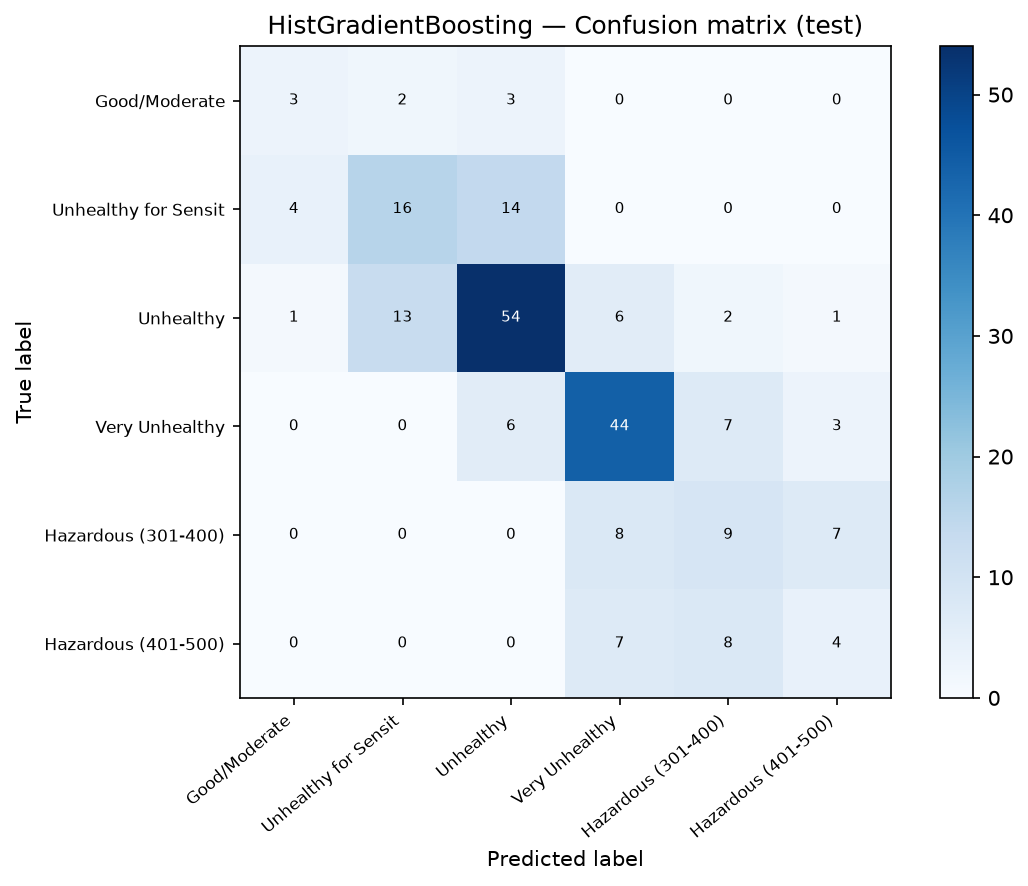
\includegraphics[width=0.82\linewidth]{classification_confusion_histgradientboosting_test.png}
  \caption{Selected HGB test confusion matrix. The raw matrix is also given in Table~\ref{tab:clf-confusion}.}
  \label{fig:clf-confusion}
\end{figure}

\begin{figure}[htbp]
  \centering
  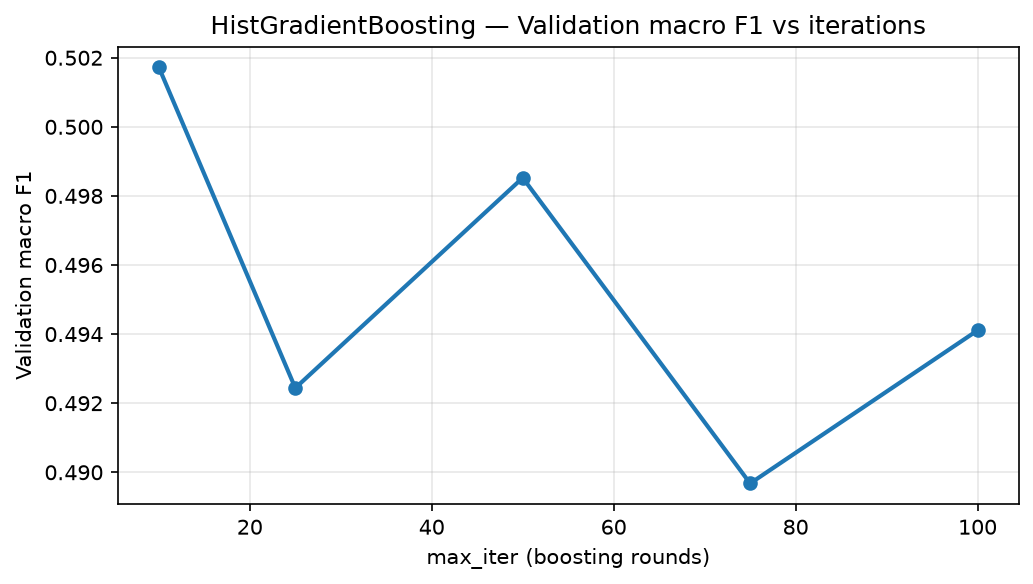
\includegraphics[width=0.82\linewidth]{classification_hgb_val_curve.png}
  \caption{Validation macro F1 for the HGB configuration used in model selection.}
  \label{fig:clf-curve}
\end{figure}

\begin{figure}[htbp]
  \centering
  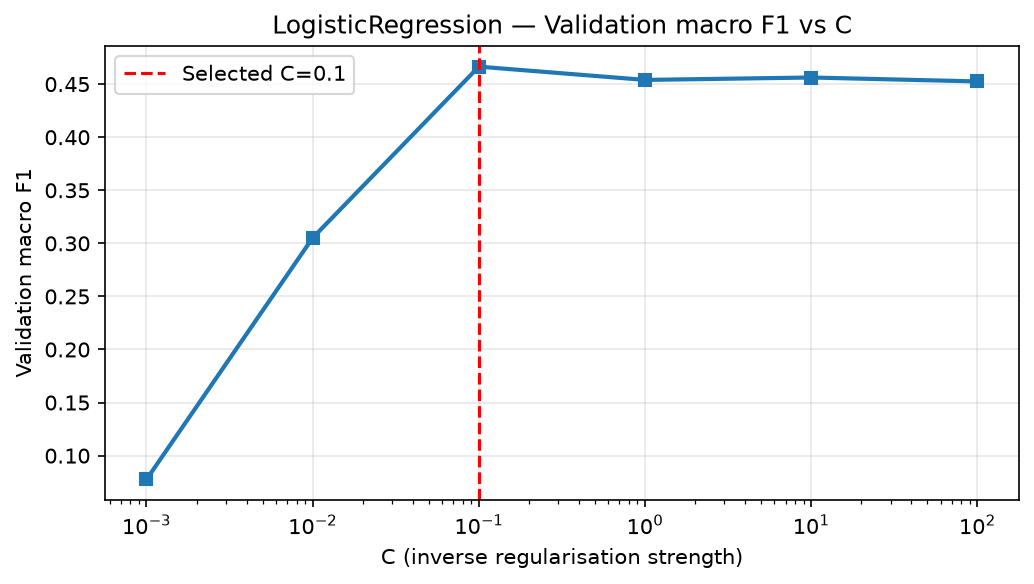
\includegraphics[width=0.78\linewidth]{classification_lr_C_curve.png}
  \caption{Logistic-regression validation curve over the regularisation strength $C$. The selected value was $C=0.1$.}
  \label{fig:clf-c}
\end{figure}

\paragraph{Training curves.} A per-epoch training-loss curve exists only for the MLP, which was excluded because its validation macro F1 (0.4124) did not exceed that of HGB (0.4941). For logistic regression (full-batch solver) and HGB (no per-epoch loss recorded in our configuration) we report validation-score curves instead (Figures~\ref{fig:clf-curve}, \ref{fig:clf-c}, and \ref{fig:reg-learning}). Figure~\ref{fig:clf-curve} is nearly flat (macro F1 between about 0.490 and 0.502), so the iteration count is not a sensitive parameter.

\section{Phase 3: Regression results}
\label{sec:reg-results}

Table~\ref{tab:reg-metrics} reports the regression comparison. On validation, HGB had the lowest RMSE (45.6243), narrowly ahead of Ridge (45.6916); both beat persistence (51.5457) by about 11.4--11.5\%. On test, however, HGB reached 64.9198, essentially tied with persistence (64.8175, a 0.10 RMSE gap); its skill score was $-0.0016$. Ridge reached 62.0956 on test and beat persistence, with skill 0.0420. R2 follows the same pattern: Ridge's test $R^2$ is 0.7356, HGB's is 0.7110, and persistence's is 0.7119.

This is a genuine validation-to-test reversal, not a reporting error. The selection rule chose HGB on validation RMSE before test was touched. The report keeps that selection and reports the test outcome honestly. It does not switch the final model to Ridge after seeing test.

\begin{table}[htbp]
\centering
\small
\caption{Regression results on the chronological validation and test splits. Skill is $1-\mathrm{RMSE}_{model}/\mathrm{RMSE}_{persistence}$.}
\label{tab:reg-metrics}
\begin{tabular}{llrrrrr}
\toprule
Model & Split & RMSE & MAE & $R^2$ & Skill & $n$ \\
\midrule
Persistence & Validation & 51.5457 & 33.5298 & 0.7808 & -- & 244 \\
Persistence & Test & 64.8175 & 39.9777 & 0.7119 & -- & 222 \\
Ridge & Validation & 45.6916 & 31.8794 & 0.8277 & 0.1136 & 244 \\
Ridge & Test & 62.0956 & 38.4750 & 0.7356 & 0.0420 & 222 \\
\textbf{HGB} & Validation & 45.6243 & 29.9781 & 0.8282 & 0.1149 & 244 \\
\textbf{HGB} & Test & 64.9198 & 40.7740 & 0.7110 & -0.0016 & 222 \\
\bottomrule
\end{tabular}

\end{table}


All models are scored on the same 244 validation and 222 test scorable rows; the 6 validation and 1 test rows dropped for missing current-day PM2.5 are not scored.

\begin{figure}[htbp]
  \centering
  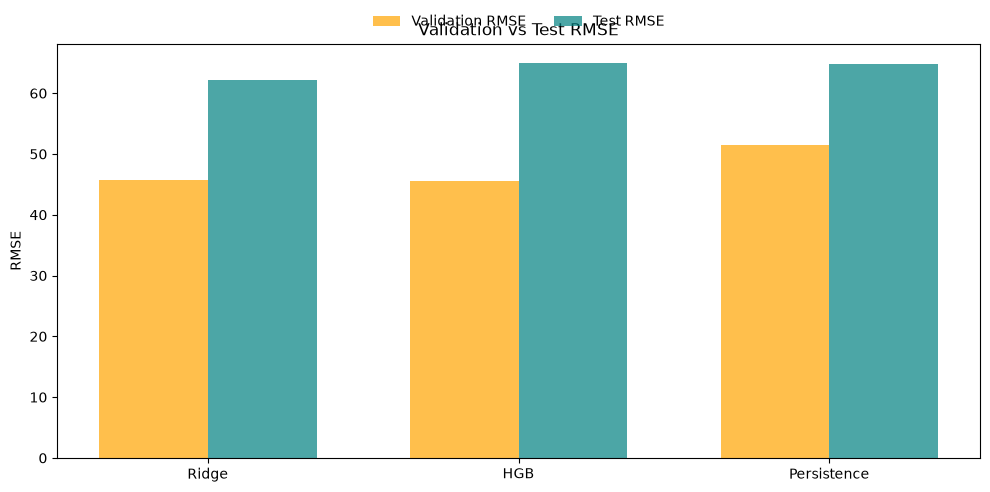
\includegraphics[width=0.82\linewidth]{regression_metric_comparison.png}
  \caption{Regression metric comparison across candidate models and splits.}
  \label{fig:reg-comparison}
\end{figure}

\begin{figure}[htbp]
  \centering
  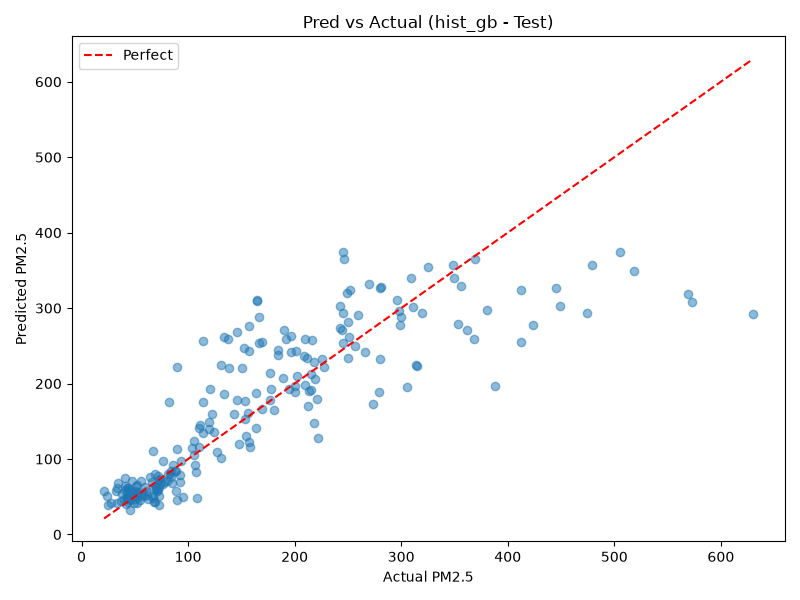
\includegraphics[width=0.9\linewidth]{regression_hist_gb_pred_vs_actual.png}
  \caption{Selected HGB regression: predicted versus actual next-day PM2.5.}
  \label{fig:reg-pred}
\end{figure}

\begin{figure}[htbp]
  \centering
  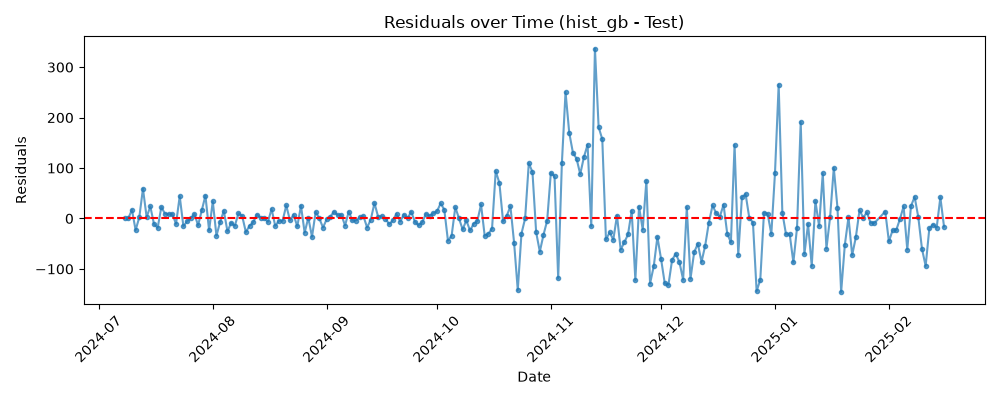
\includegraphics[width=0.9\linewidth]{regression_hist_gb_residuals_over_time.png}
  \caption{Selected HGB regression residuals over time.}
  \label{fig:reg-resid-time}
\end{figure}

\begin{figure}[htbp]
  \centering
  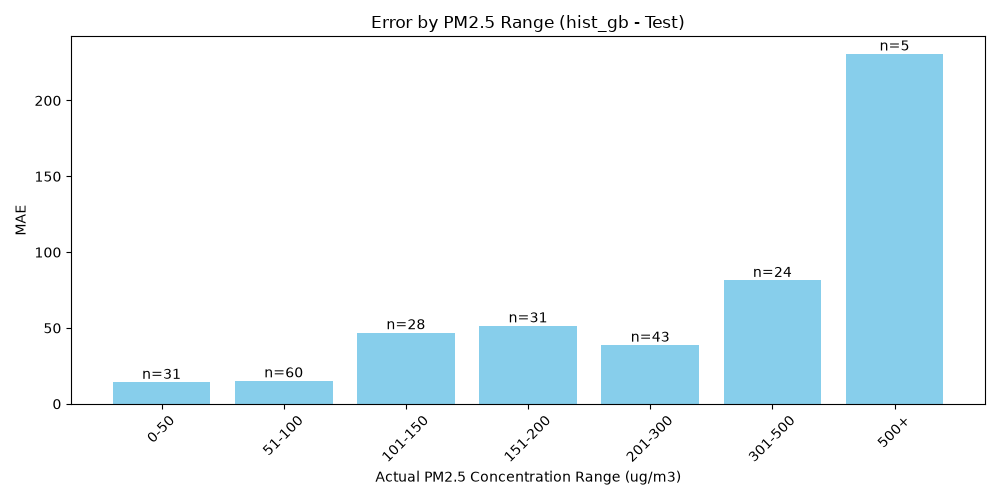
\includegraphics[width=0.82\linewidth]{regression_hist_gb_error_by_severity.png}
  \caption{Selected HGB regression error by pollution severity.}
  \label{fig:reg-severity}
\end{figure}

\begin{figure}[htbp]
  \centering
  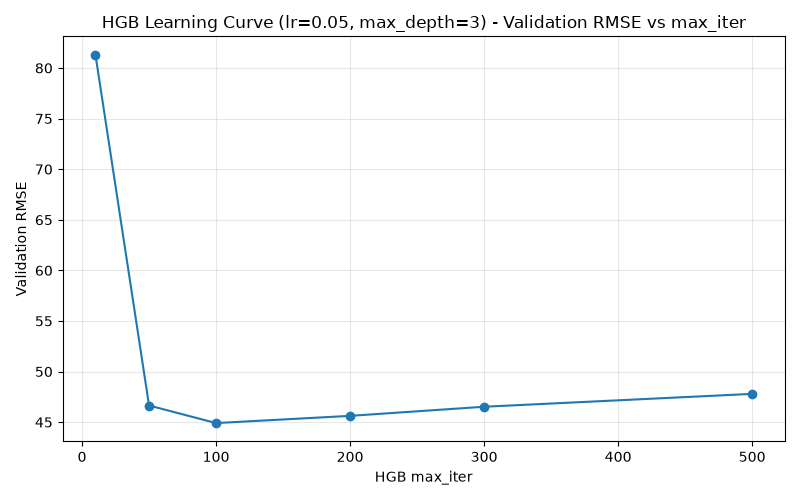
\includegraphics[width=0.82\linewidth]{regression_hgb_learning_curve.png}
  \caption{HGB regression learning curve used as training diagnostic material.}
  \label{fig:reg-learning}
\end{figure}

\section{Phase 4: Bias and error analysis}

The bias analysis joins the final regression and classification predictions on date and split. It uses 466 joined rows: 244 validation and 222 test. The subgroup table has 47 rows across seven dimensions: AQI category, season, year, weekday versus weekend, Islamic events, public holidays, and PM2.5 severity band. Missing subgroup keys were counted per split and dimension; all counts were zero in the final join.

The joined validation rows contain 25 scorable Ramadan rows and no scorable Eid rows. The feature table flags Eid on 10--12 April and 17--19 June 2024, but the AQI label is missing on those dates; all six dates also lack a next-day target, so they never enter the split. This is a label-coverage limitation, not a calendar-flag gap. The test split has only one Islamic-event group, \texttt{Normal}; no test Ramadan or Eid comparison is therefore possible. Public-holiday test rows number only seven, so the holiday result is marked as small-support. The analysis is environmental and temporal, not demographic: the dataset has one monitoring station and no demographic attributes. It cannot establish fairness across people or neighbourhoods.

\begin{table}[htbp]
\centering
\small
\caption{Missing subgroup keys after joining regression and classification predictions.}
\label{tab:bias-missing}
\begin{tabular}{lrr}
\toprule
Dimension & Validation missing & Test missing \\
\midrule
AQI Category & 0 & 0 \\
Islamic\_Event & 0 & 0 \\
Public\_Holiday & 0 & 0 \\
Season & 0 & 0 \\
Severity\_Band & 0 & 0 \\
Weekday\_Weekend & 0 & 0 \\
Year & 0 & 0 \\
\bottomrule
\end{tabular}

\end{table}


Table~\ref{tab:bias-test} reports the test subgroups. Positive signed error is $y_{true}-y_{pred}$, so a positive value means under-prediction relative to the observed PM2.5. The most important pattern is the severe-pollution tail. Hazardous 401--500 has RMSE 162.14 and signed error 141.70; the 301--500 severity band has RMSE 99.60 and signed error 75.72; and the 500+ band, with only five rows, has RMSE 242.00 and signed error 230.76. These are large errors, not just noise, although the 500+ estimate is unstable because of its tiny support. Severity bands and AQI-category groups are defined by the observed outcome, so high-severity groups look under-predicted and low-severity groups over-predicted partly by construction. The size of the errors (for example RMSE 99.60 on the 301--500 band), not the sign, is the informative result.

Seasonal errors are also uneven. Winter test RMSE is 72.38 with signed error $-17.43$, indicating average over-prediction, while autumn RMSE is 75.32 with signed error $+14.15$, indicating average under-prediction. Summer is much easier (RMSE 19.65). Test 2025 has only 45 rows (1 January--16 February, winter), whereas 2024 has 177 mixed-season rows. The 2025 comparison is therefore confounded with season: RMSE is 69.86 versus 63.60, and macro F1 is 0.4306 versus 0.4832, but this is not a clean temporal comparison. Weekday RMSE is higher than weekend RMSE (68.32 versus 55.64), though weekend macro F1 is lower (0.4276 versus 0.4875).

{\footnotesize
\setlength{\tabcolsep}{4pt}
\begin{longtable}{@{}llrrrrrr@{}}
\caption{Test-set subgroup error and classification performance. Positive signed error means the true value is above the prediction (under-prediction). Small-support groups are marked with $^{*}$.}\label{tab:bias-test}\\
\toprule
Dimension & Group & $n$ & RMSE & MAE & Signed err. & Acc. & Macro F1 \\
\midrule
\endfirsthead
\toprule
Dimension & Group & $n$ & RMSE & MAE & Signed err. & Acc. & Macro F1 \\
\midrule
\endhead
AQI Category & Good/Moderate$^{*}$ & 8 & 25.4601 & 23.6583 & -23.6583 & 0.3750 & 0.5455 \\
AQI Category & Unhealthy for Sensitive & 34 & 12.5892 & 9.8540 & -7.1164 & 0.4706 & 0.6400 \\
AQI Category & Unhealthy & 77 & 43.8019 & 27.9535 & -11.1751 & 0.7013 & 0.8244 \\
AQI Category & Very Unhealthy & 60 & 59.1430 & 44.7748 & -27.9941 & 0.7333 & 0.8462 \\
AQI Category & Hazardous (301-400)$^{*}$ & 24 & 53.2085 & 41.5136 & 11.8486 & 0.3750 & 0.5455 \\
AQI Category & Hazardous (401-500)$^{*}$ & 19 & 162.1417 & 141.6998 & 141.6998 & 0.2105 & 0.3478 \\
Season & Winter & 76 & 72.3755 & 52.6206 & -17.4306 & 0.6053 & 0.4494 \\
Season & Summer & 55 & 19.6486 & 15.0855 & 0.7674 & 0.5091 & 0.4763 \\
Season & Autumn & 91 & 75.3234 & 46.4062 & 14.1519 & 0.6154 & 0.4358 \\
Year & 2024 & 177 & 63.6013 & 39.2136 & 0.7755 & 0.5763 & 0.4832 \\
Year & 2025 & 45 & 69.8649 & 46.9118 & -2.9323 & 0.6222 & 0.4306 \\
Weekday\_Weekend & Weekday & 158 & 68.3224 & 41.7848 & 1.0546 & 0.6139 & 0.4875 \\
Weekday\_Weekend & Weekend & 64 & 55.6356 & 38.2786 & -2.5206 & 0.5156 & 0.4276 \\
Severity\_Band & 0-50 & 31 & 17.6658 & 14.2902 & -12.6398 & 0.4839 & 0.5386 \\
Severity\_Band & 51-100 & 60 & 26.2778 & 15.2874 & 1.1969 & 0.6333 & 0.5302 \\
Severity\_Band & 101-150$^{*}$ & 28 & 61.8758 & 47.0172 & -34.7032 & 0.7143 & 0.8333 \\
Severity\_Band & 151-200 & 31 & 66.9282 & 51.5369 & -42.0886 & 0.8387 & 0.9123 \\
Severity\_Band & 201-300 & 43 & 50.0110 & 38.7876 & -8.5917 & 0.5349 & 0.5635 \\
Severity\_Band & 301-500$^{*}$ & 24 & 99.6015 & 81.4907 & 75.7243 & 0.2083 & 0.2556 \\
Severity\_Band & 500+$^{*}$ & 5 & 242.0043 & 230.7646 & 230.7646 & 0.6000 & 0.7500 \\
Islamic\_Event & Normal & 222 & 64.9198 & 40.7740 & 0.0239 & 0.5856 & 0.4780 \\
Public\_Holiday & Normal & 215 & 65.6586 & 41.4275 & -0.3726 & 0.5767 & 0.4680 \\
Public\_Holiday & Holiday$^{*}$ & 7 & 35.3757 & 20.7040 & 12.2017 & 0.8571 & 0.7333 \\
\bottomrule
\end{longtable}
}


\noindent{\footnotesize\textit{Table note:} Subgroup macro F1 is computed within each subgroup over the true classes present, so it is not comparable across groups or with Table~\ref{tab:clf-metrics}. For AQI Category rows, use accuracy (= recall).\par}

\begin{figure}[htbp]
  \centering
  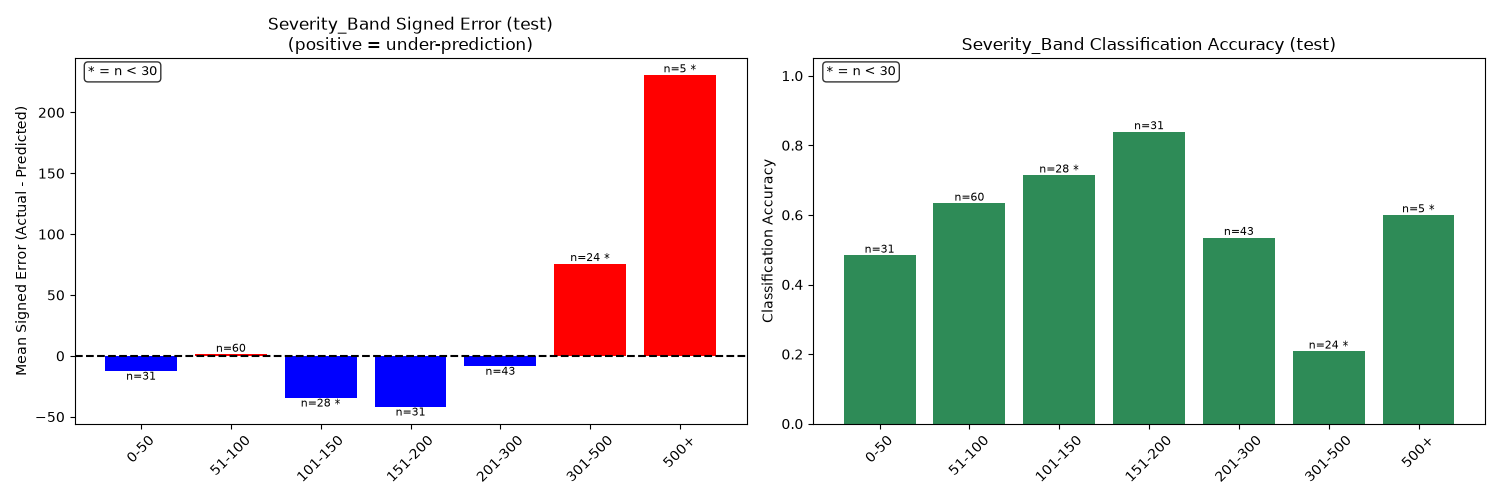
\includegraphics[width=0.95\linewidth]{bias_Severity_Band_test.png}
  \caption{Test signed error and classification accuracy by PM2.5 severity band. Because groups are defined by the observed outcome, the sign is partly constructed; the error magnitude is the informative result. Small groups are marked with an asterisk.}
  \label{fig:bias-severity}
\end{figure}

\begin{figure}[htbp]
  \centering
  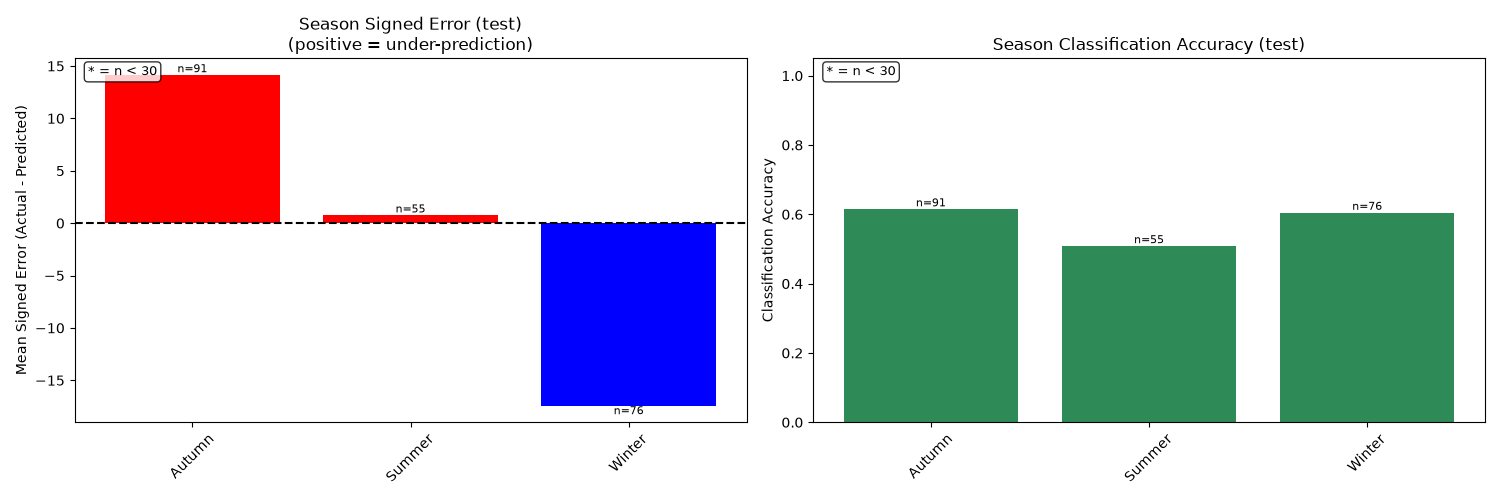
\includegraphics[width=0.95\linewidth]{bias_Season_test.png}
  \caption{Test signed error and classification accuracy by season.}
  \label{fig:bias-season}
\end{figure}

\begin{figure}[htbp]
  \centering
  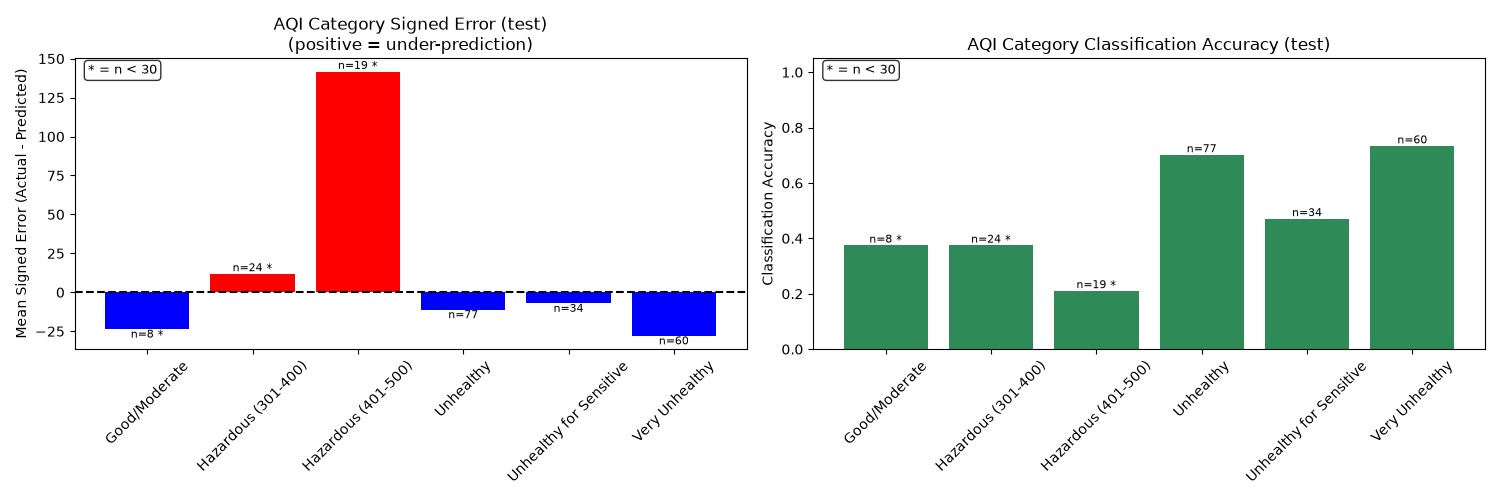
\includegraphics[width=0.95\linewidth]{bias_AQI_Category_test.png}
  \caption{Test signed error and classification accuracy by observed AQI category.}
  \label{fig:bias-aqi}
\end{figure}

\begin{figure}[htbp]
  \centering
  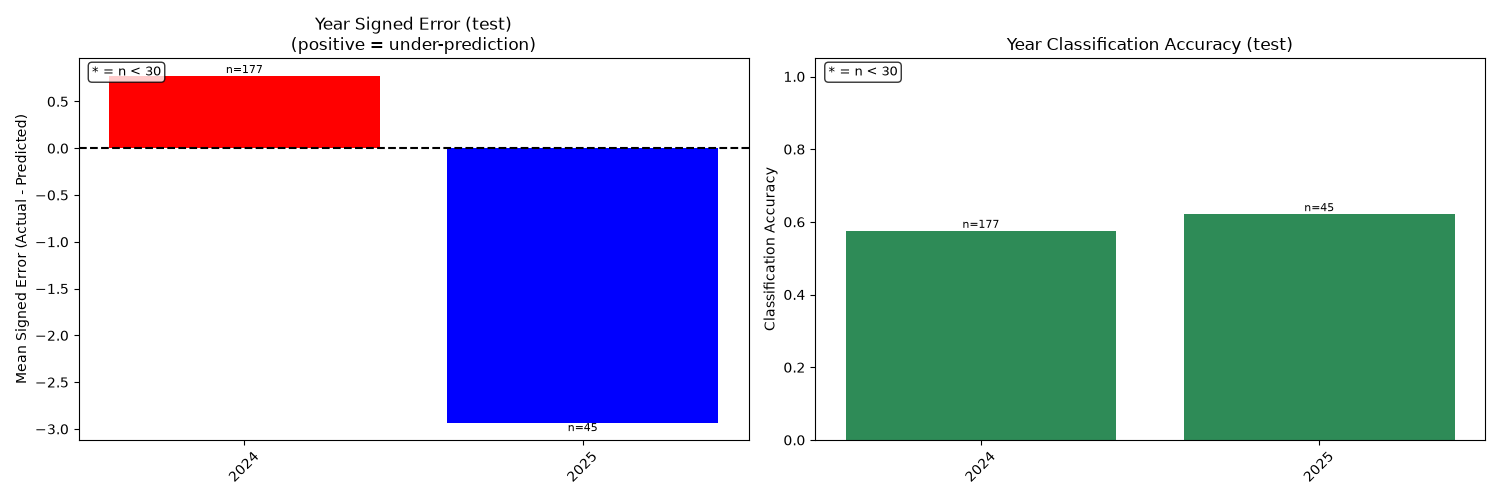
\includegraphics[width=0.95\linewidth]{bias_Year_test.png}
  \caption{Test signed error and classification accuracy by year.}
  \label{fig:bias-year}
\end{figure}

\begin{figure}[htbp]
  \centering
  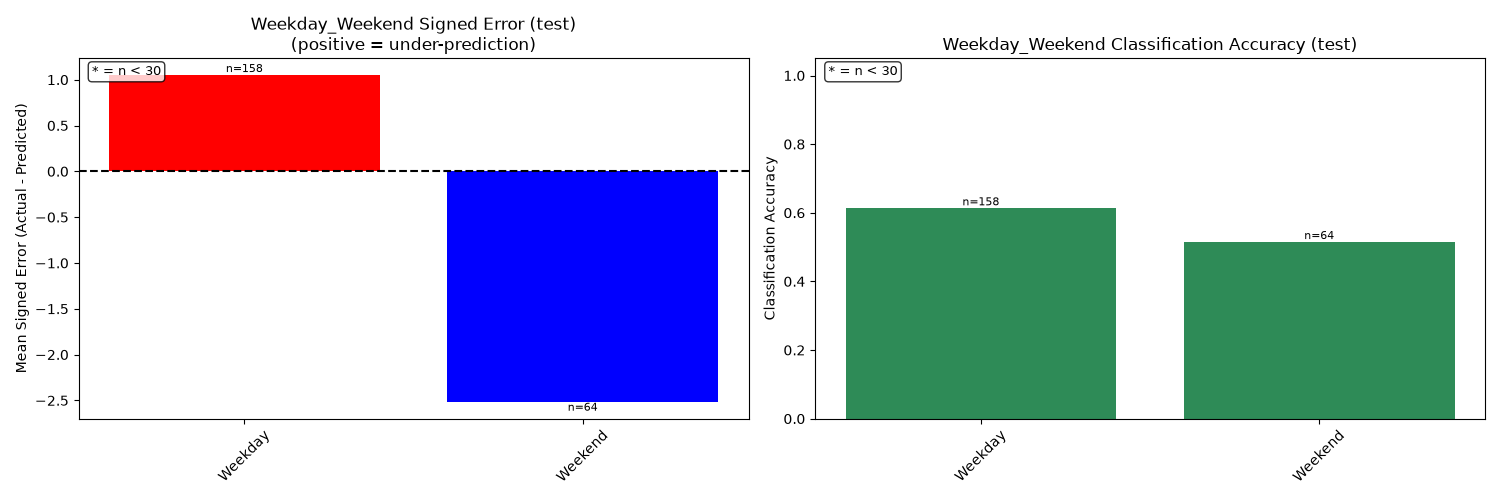
\includegraphics[width=0.95\linewidth]{bias_Weekday_Weekend_test.png}
  \caption{Test signed error and classification accuracy for weekday versus weekend rows.}
  \label{fig:bias-weekday}
\end{figure}

\begin{figure}[htbp]
  \centering
  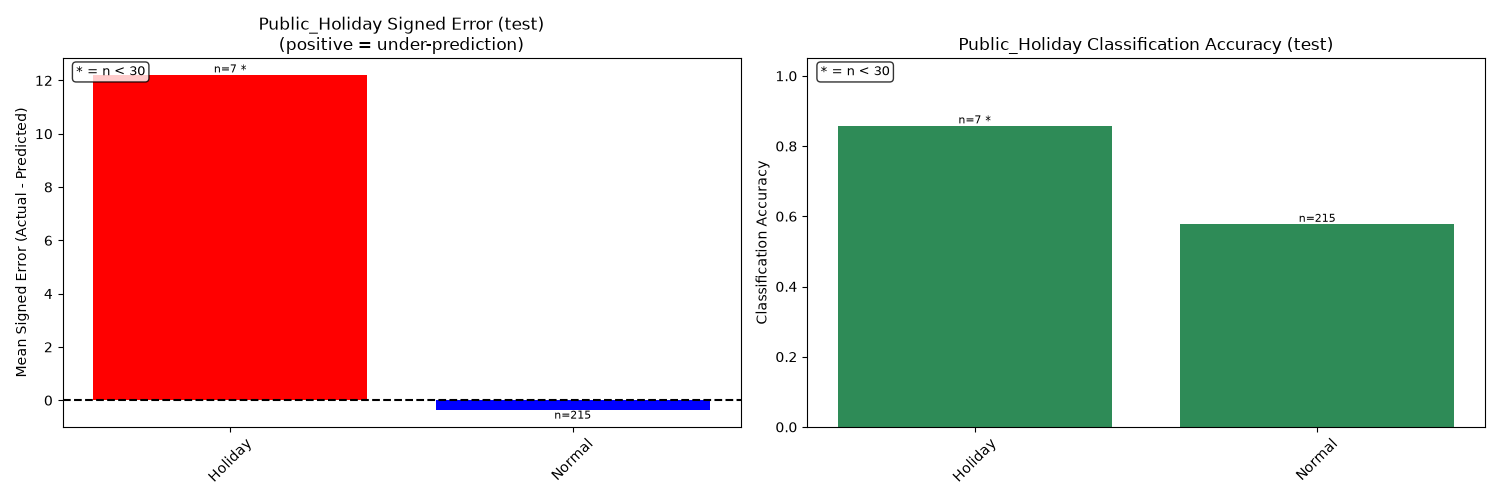
\includegraphics[width=0.95\linewidth]{bias_Public_Holiday_test.png}
  \caption{Test signed error and classification accuracy for normal days versus public holidays. Holiday support is only seven rows.}
  \label{fig:bias-holiday}
\end{figure}

The full set of 14 bias charts (seven dimensions for validation and test) is included in the \texttt{figures/} folder. The charts mark groups with $n<30$ with an asterisk; those estimates should not be read as precise.

The class mix also shifts across periods. Unhealthy is about 48\% of training rows but 32\% of validation and 35\% of test. The two Hazardous bands together are about 10\% of training but 22\% of validation and 19\% of test. This may reflect seasonal composition, missing training days or targets, or real worsening; the data do not identify a single cause. The later-period under-prediction of severe days is consistent with that shift, but it is not proof of a causal trend.

\section{Phase 4: Limitations and recommendations}

\begin{itemize}[leftmargin=1.4em]
  \item \textbf{Rare-class uncertainty.} Good/Moderate has 8 test rows and Hazardous 401--500 has 19. Their per-class precision/recall are noisy. The same applies to small bias subgroups such as public holidays and the 500+ severity band.
  \item \textbf{Single station.} The dataset represents one monitoring location and has no demographic attributes. The bias check cannot support claims about population-level fairness.
  \item \textbf{Distribution shift.} The class mix and the validation-to-test error pattern change over time. A model selected on validation can fail to beat persistence on a later period, as happened on both tasks (macro F1 below persistence for classification, and essentially tied on RMSE for regression).
  \item \textbf{Coverage gaps.} The validation split contains 250 usable rows over the 326 days from 2023-07-14 to 2024-06-03 (about 77\%), because many days lack an AQI label or a next-day target; the test split has 223 rows over the 224 days from 2024-07-08 to 2025-02-16 and contains no spring rows. Validation and test therefore cover different seasonal mixes, which limits how directly their metrics can be compared.
  \item \textbf{Macro F1 versus accuracy.} HGB's test accuracy is higher than persistence's, but its macro F1 is lower. Reporting only accuracy would obscure the rare-class weakness.
  \item \textbf{No traffic data.} Calendar features are proxies; no open, time-aligned Lahore traffic dataset was available. This limits the explanatory scope of the features.
  \item \textbf{No test-time retuning.} The report preserves the validation-based selection. Switching to Ridge after seeing test would be post-hoc and would invalidate the test-once rule.
\end{itemize}

Recommended next steps are to collect more severe-pollution days, evaluate cost-sensitive or class-balanced variants with a pre-registered validation rule, add calibrated probabilities and prediction intervals, and test on a later period or a second station. Any such change should be selected without using the current test set.

\section{Phase 4: Reproducibility}

The final results were produced from merge commit \texttt{a55a7f5} on \texttt{main}; the repository README was updated afterwards (commit \texttt{56dea73}). The final pipeline was run from the repository root with:

\begin{verbatim}
python -m src.check_setup
python -m unittest discover -s tests -t .
python -m src.classification
python -m src.regression
python -m src.bias_analysis
\end{verbatim}

\texttt{check\_setup} reported 0 bad next-day PM2.5 values, 0 bad lag-1 values, and 0 bad next-day categories. The unit tests ran 15 tests and passed. Classification completed in 427.92 seconds and regression in 37.61 seconds. The bias analysis then joined the final prediction files.

The classification prediction file has 473 rows and 12 columns; 466 rows are scorable. Its SHA-256 hash is \texttt{47D8E0A89FC3F37EA6B74E807DCF566FBDD6D79F734D5A05CFD56124888EB2EB}, matching the verified Drive copy. Regression also has 473 prediction rows, 466 scorable.

Dependencies are listed in \texttt{requirements.txt}. The final environment used pandas 3.0.3, scikit-learn 1.9.1, and matplotlib 3.11.2. The seed is 42 from \texttt{configs/base.yaml}. Generated prediction CSVs, metrics JSON, and charts are review artifacts and should not be committed to Git; the data and large artifacts belong on the shared Drive or a release link. No fitted model weights are published: the selected pipelines are refit from fixed seeds by the committed scripts (see the repository README).

\subsection{Git-author contributions}

Table~\ref{tab:git-authors} is the Git-author contribution table: it maps each commit author to the project modules and representative commits they own. The repository history contains only the three project contributors. The Git identities used in the D2 work are Abdul Rehman \texttt{<}\url{arehman4275@gmail.com}\texttt{>}, Muhammad Haider Mughal \texttt{<}\url{haiderirfanmm@gmail.com}\texttt{>}, and Muhammad Ayub Butt \texttt{<}\url{purestudy83010@gmail.com}\texttt{>}. Some earlier commits by the same author also appear under the display name ``Haider Mughal'' with the same e-mail address. No AI or OpenCode co-author trailer was added.

\begin{table}[htbp]
\centering
\footnotesize
\caption{Git-author contribution table: commit authors mapped to project modules. The package and report list exactly the three human project contributors.}
\label{tab:git-authors}
\begin{tabular}{llL{4.5cm}L{4.9cm}}
\toprule
Contributor & ID & D2 contribution & Key modules and representative commits \\
\midrule
Abdul Rehman & 3059 & Shared data and evaluation foundation; integration; D2 report & \texttt{src/data.py}; \texttt{src/evaluate.py}; \texttt{src/check\_setup.py}; \texttt{configs/base.yaml}; \texttt{tests/test\_evaluate.py}; \texttt{reports/} (\texttt{b672bfc}, \texttt{20fa79e}, \texttt{a55a7f5}) \\
Muhammad Haider Mughal & 3006 & Classification pipeline and tuning & \texttt{src/classification.py} (\texttt{d311f8e}, \texttt{5f57987}) \\
Muhammad Ayub Butt & 3076 & Regression and bias analysis & \texttt{src/regression.py}; \texttt{src/bias\_analysis.py} (\texttt{fae7490}, \texttt{6e2448d}) \\
\bottomrule
\end{tabular}
\end{table}


\section{Phase 4: Conclusion}

The primary classification model, HGB, was selected on validation macro F1 and reached 0.4780 on test. It did not beat persistence's 0.5157 macro F1, even though its accuracy was slightly higher. The secondary regression model, HGB, was selected on validation RMSE only; test results were not used to change the selection. Its test RMSE was 64.9198, essentially tied with persistence's 64.8175 (a 0.10 gap and skill $-0.0016$). Ridge did beat persistence on test with RMSE 62.0956, but switching to it after seeing test would violate the validation-only selection rule. The bias analysis shows that the largest error magnitudes occur on the most severe pollution days; because those groups are defined by the observed outcome, the sign is partly constructed, so the magnitude is the informative result. Seasonal and temporal errors are also uneven. These results are reported as observed, without retuning on the test set.

\begin{thebibliography}{9}

\bibitem{epa_aqi}
U.S. Environmental Protection Agency,
``Technical Assistance Document for the Reporting of Daily Air Quality -- the Air Quality Index (AQI),'' EPA-454/B-18-007, September 2018.

\bibitem{who2024ambient}
World Health Organization,
``Ambient (outdoor) air pollution,'' fact sheet, 24 October 2024.

\bibitem{lahore}
R. Majeed, M. S. Anjum, M. Imad-ud-din, S. Malik, M. N. Anwar, B. Anwar, and M. F. Khokhar,
``Solving the mysteries of Lahore smog: the fifth season in the country,''
\emph{Frontiers in Sustainable Cities}, vol. 5, art. 1314426, 2024.

\bibitem{scikit}
F. Pedregosa et al.,
``Scikit-learn: Machine Learning in Python,''
\emph{Journal of Machine Learning Research}, vol. 12, pp. 2825--2830, 2011.

\bibitem{hgb}
J. H. Friedman,
``Greedy Function Approximation: A Gradient Boosting Machine,''
\emph{Annals of Statistics}, vol. 29, no. 5, pp. 1189--1232, 2001.

\end{thebibliography}

\end{document}
